\documentclass[10pt, conference, letterpaper]{IEEEtran}
\usepackage{cite}
\usepackage{xcolor,soul,framed}
\usepackage{amsmath,amsthm,amssymb,amsfonts}
\usepackage{algorithmic}
\usepackage{graphicx}
\usepackage{color, soul}
\usepackage{algorithm, algorithmic}
\usepackage[utf8]{inputenc}
\usepackage[english]{babel}
\usepackage{mathtools}
\graphicspath{ {./images/} }

%---------------------------------------------------------------%
\newtheorem{definition}{Denifition}
\newtheorem{problem}{Problem}
\newtheorem{lemma}{Lemma}
\newtheorem{corollary}{Corollary}
\newtheorem{example}{Example}
\newcommand{\domZ}{\mathbb{Z}_{*}}
\newcommand{\vecOne}{\mathbf{1}}
\newcommand{\ind}{\mathbf{I}}
\DeclarePairedDelimiter\set\{\}
%---------------------------------------------------------------%
\newcommand{\apSet}{\mathcal{K}}
\newcommand{\esSet}{\mathcal{M}}
\newcommand{\wSet}{\mathcal{W}}
\newcommand{\uSet}{\mathcal{U}}
\newcommand{\cSet}{\mathcal{C}}
\newcommand{\Stat}{\mathbf{S}}
%---------------------------------------------------------------%

\begin{document}

    %=============================== TITLE ===============================%
    \title{
        Meet-in-Future: Distributed Online Job Dispatching with Obsolete Information in Edge Computing System
    }
    \author{
        \IEEEauthorblockN{Yuncong Hong}
        \IEEEauthorblockA{
            \textit{Department of CS}, The University of Hong Kong, China \\
            ychong@cs.hku.hk
        }
    }
    \maketitle

    %============================== ABSTRACT ==============================%
    \begin{abstract}
        \label{sec:abstract}
        We formulate the problem with job dispatching in distributed Edge Computing system, and identify the difficulty exists in cooperation between APs (Access Points) and ESs (Edge Servers) with delayed information. In this work, we design the broadcast information in the system and formulate the corresponding problem into a MDP problem.
    \end{abstract}

    \begin{IEEEkeywords}
        Edge Computing, Job Dispatch, Delayed Information, Collective Observability, Distributed Multi-agent MDP
    \end{IEEEkeywords}

    %============================ INTRODUCTION ============================%
    \begin{section}{INTRODUCTION}
        \label{sec:introduction}
        (in progress)

        Some traits to mention compared to related works:
        \begin{itemize}
            \item we consider arrival process on ES may be affected by uploading process;
            \item we consider decentralized cooperation among APs without help from a centralized agent;
            \item we identify the delayed received broadcast information is un-acceptable, and it's hard to establish cooperation among APs because of obsolete information;
            \item we consider online job dispatching immediately without waiting for collective information and avoid the waiting time for decision.
        \end{itemize}
    \end{section}

    %========================= LITERATURE REVIEW ==========================%
    \begin{section}{LITERATURE REVIEW}
        \label{sec:review}
        Related work from \emph{Conference}:
        \begin{itemize}
            \item We use MDP definition in \cite{sutton1998introduction}
            \item The earliest related works we find is \cite{ref-01} (cited 167 times). In this work, the single agent is assumed not able to observe the global state, and thus they need communication to establish cooperation by sharing \emph{information}. The agent considers communication as extra action to synchronize the states and thus incurs extra cost. \\
            However, the communication is without delay, and converted into POMDP problem.
            \item The other work \cite{ref-02} considers continuous state observation with constant or stochastic delay with single agent. \\
            However, 
        \end{itemize}

        Realted work from \emph{Journal/Magazine}:
        \begin{itemize}
            \item (in progress...)
        \end{itemize}
    \end{section}

    %============================ SYSTEM MODEL ============================%
    \begin{section}{SYSTEM MODEL}
        \label{sec:model}
        \begin{subsection}{Network Model}
            The network topology of the MEC system considered is illustrated in Fig. \ref{fig:system}, which is composed of three elements. The user equipment (UE) is connected to its corresponding access point (AP), and .The AP provides network access and accepts the computing jobs released to all the UEs connected, but AP itself is assumed to have no computation capability because it could not carry various computation resources for various jobs. So, AP would upload the job computation request to the backend edge servers (ES) and the dispatch decision should be made on APs to determine which server to select.
            \begin{figure}[ht]
                \centering
                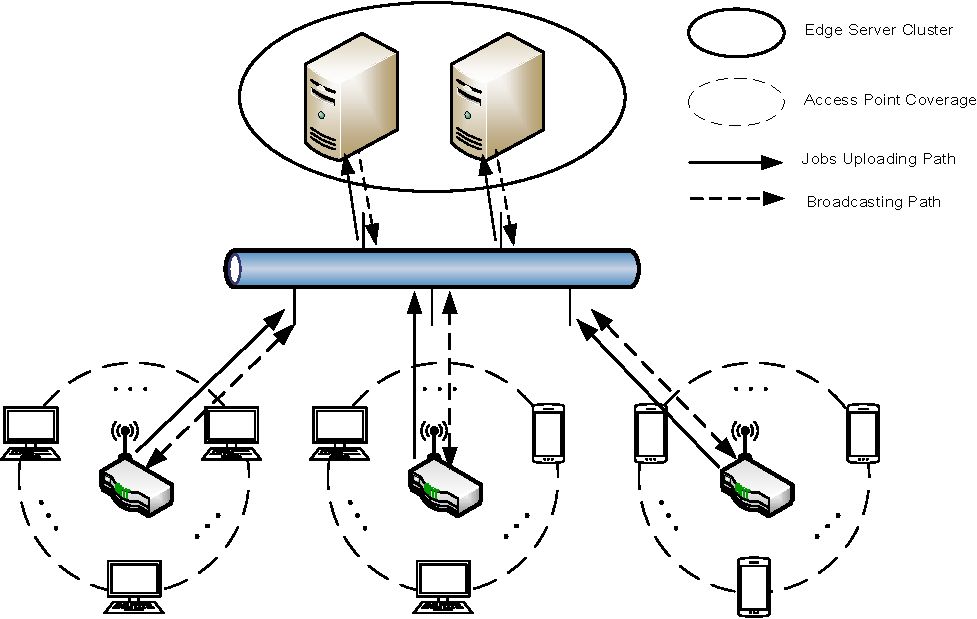
\includegraphics[width=0.45\textwidth, trim={0.5cm 0.5cm 0.5cm 0.5cm}, clip]{system-model.pdf}
                \caption{The Illustration of MEC System Model}
                \label{fig:system}
            \end{figure}

            Let $\mathcal{K} \triangleq \set{1,\dots,K}$ and $\mathcal{M} \triangleq \set{1,\dots,M}$ denote the set of APs and set of ESs in the MEC system respectively. We adapt \emph{timeslot} as the minimum time slice in the system, where the job release behavior from UEs under $k$-th AP is considered time-invariant in each timeslot.
            \begin{itemize}
                \item \emph{Waiting Job Set} on $k$-th AP node in $t$-th timeslot as: $\wSet_{k}(t) = \set{w_1, w_2, \dots, w_{N^w_k(t)}}, \forall k \in \apSet$; where $w_i \in \domZ^M$ denotes the computing length on all $M$ unrelated edge servers.
                \item \emph{Uploading Job Set} from $k$-th AP to $m$-th ES in $t$-th timeslot as: $\uSet_{k,m}(t) = \set{u_1, u_2, \dots, u_{N^u_{k,m}(t)}}, \forall k \in \apSet, m \in \esSet$; where $u_i \in (L_C), L_{cd}^{(U)}(t)$.
                \item \emph{Computing Job Set} on $m$-th ES in $t$-th timeslot as: $\cSet_{m}(t) \triangleq \set{L_{cd}^{(C)}(t)}$;
            \end{itemize}

            Furthermore, we consider there is at most one job arrives AP in one timeslot and we characterize the job release process to AP with \emph{Bernoulli process} to characterize the memory-less behavior and there could be at most one job arrives in one timeslot.

            (For Communications) We identify \emph{delay} as the most unacceptable part in MEC system; well-designed broadcast to help APs come to consensus on global states;
            \begin{itemize}
                \item for \emph{Parallel Uploading}: because the uploading time is finite and arrival frequency is at most 1 per timeslot, there actually needs finite channel capacity to serve the uploading process;
                \item The total uploading process could be divided into Fig. \ref{fig:trans} between the adjacent timeslots, using some \emph{indicator functions};
            \end{itemize}

            While the jobs processing is carried out following a descriptive procedure in the model section, we need some denotations to characterize the intrinsic of the transition. Firstly We come up with denotations for transition job sets expressed in figure \ref{fig:trans} as:
            \begin{align}
                I^{(W \to W')}_{k}(t) & \triangleq \{ j | a^{(k)}(j)=0, \forall j \in S^{'(W)}_k(t)\}
                \\
                I^{(W \to U)}_{k,n}(t) &\triangleq \{ j | a^{(k)}(j)=n, \forall j \in S^{'(W)}_k(t)\}
                \\
                I^{(U \to C)}_{k,n}(t) &\triangleq \{j|(L^{(U)}_{cd})_j=1, \forall j \in S^{(U)}_{k,n}(t)\}
                \\
                I^{(U \to U')}_{k,n}(t) &\triangleq S^{(U)}_{k,n}(t) \backslash I^{(U \to C)}_{k,n}(t)
                \\
                I^{(C \to \Phi)}_{n}(t) &\triangleq \{j|\arg\min_{j} (L^{(C)}_{cd})_j \wedge (L^{(C)}_{cd})_j=1\}
                \\
                I^{(C \to C')}_{n}(t) &\triangleq S^{(C)}_{n}(t) \backslash I^{(C \to \Phi)}_{n}(t)
            \end{align}
            \begin{figure}[h]
                \centering
                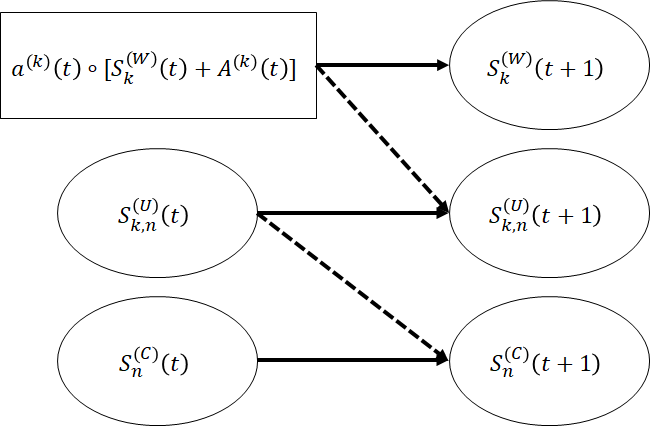
\includegraphics[width=0.45\textwidth]{single-transition.png}
                \caption{Single-step transition function composing graph}
                \label{fig:trans}
            \end{figure}
            Then we establish the relationship between those indicator functions with $S(t+1)$:
            \begin{align}
                \begin{cases}
                    S^{(W)}_{k}(t+1) = I^{(W \to W')}_{k}(t)
                    \\
                    S^{(U)}_{k,n}(t+1) = I^{(W \to U)}_{k,n}(t) + I^{(U \to U')}_{k,n}(t)
                    \\
                    S^{(C)}_{n}(t+1) = \sum_k I^{(U \to C)}_{k,n}(t) + I^{(C \to C')}_{n}(t)
                \end{cases}
            \end{align}
        \end{subsection}

        \begin{subsection}{Computation Model}
            unrelated machine model \cite{tan-online}, job length to characterize the resource preparation;
            job length bounded by $L_C$;
            resource available is known because shared cooperation at initialization phase;
            deterministic rate and only one job at one time at servers' side;
            job scheduling policy on all the server is identical.
        \end{subsection}

        \begin{subsection}{Broadcast Model}
            \begin{itemize}
                \item time scale elaboration
                \item global aligned broadcast, and interval is far larger than the maximum delay from one nodes to the other AP nodes, i.e. $T \gg d$;
                \item consensus delay for $k$-th AP:
                    \begin{align}
                        \hat{d}_k = \max_{i\in(\mathcal{K} \cup \mathcal{N})}(d_{k,i})
                    \end{align}
            \end{itemize}
            The illustration figure \ref{fig:brd} for single broadcast includes several important time points which are also important in multiple synchronous broadcast: $x_{k,j}, d_{k,j}, T^{br}_{k,j}$
            \begin{figure}[ht]
                \centering
                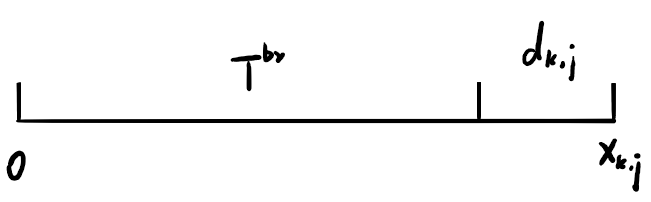
\includegraphics[width=0.45\textwidth]{single-broadcast.png}
                \caption{Single broadcast timing illustration}
                \label{fig:brd}
            \end{figure}
            And with the implication from the single broadcast, we generalize the conclusion for every broadcasts with:
            \begin{align}
                x_{k,j} = d_{k,j} + T^{br}_{j}
            \end{align}
            which takes a reasonable assumption that $T>d$ always ($j=k',n$ for $k$-th AP).
        \end{subsection}
    \end{section}

    %============================ FORMULATION =============================%
    \begin{section}{FORMULATION}
        \label{sec:formulation}
        \begin{section}{System State and Scheduling Policy}
            We formulate the standard MDP problem in this section; a fully distributed way.

            \begin{definition}
                (System State).
                $T_t = (\Stat_t, \Stat_{t-1}, C_t)$, $t=1,2,\dots$; where the transition for $(S_{t}, S_{t-1})$ is with policy $\vec{\Omega}(\tilde{S}_i)$ elaborated in the last section.
            \end{definition}

            \begin{definition}
                (Scheduling Policy).
                Same as the definition in last section.
                \begin{align}
                    \vec{\Omega}(T_t) = \vec{\Omega}(\tilde{S}_t) \equiv \vec{\Omega}_{\Delta{t}}(S_t, S_{t-1})
                \end{align}
            \end{definition}
        \end{section}

        \begin{subsection}{The Optimization Problem}
            In our problem, we consider \emph{response time} of jobs;
            While $C_t$ denotes the cost collected in the last broadcast interval, we have the expression as:
            \begin{align}
                C_t = \sum_{t'\in[1,T^{br}]} \sum_{s'} P_{S_{t-1},s'}^{t'}(\vec{\beta}_{\Delta{t}}) \times |s'|
            \end{align}
            where,
            \begin{align}
                P_{S_{t-1},s'}^{t'}(\vec{\beta}_{\Delta{t}})
                = \{
                    \prod_{\Delta{t} \in [1,t']} P_{ss'}(\vec{\beta}_{\Delta{t}})
                \}_{S_{t-1}, s'}
            \end{align}
            
            \begin{problem}
                (Distributed Cooperative Job Dispatching)
                \begin{gather}
                    \min_{\Omega} \lim_{T \to \infty} E[\frac{1}{T} \sum_{t=0}^{T} N(t)]
                    \nonumber\\
                    N(t) = \sum_{k \in K} (A^{(k)}(t) + N_k(t))
                            + \sum_{n \in N} N_n(t)
                \end{gather}
            \end{problem}
            where $N_k(t)$ denotes the number of jobs on $k$-th AP, and $N_n(t)$ denotes the number of jobs on $n$-th ES.
            The goal to minimize the cost caused by ESs could be simply achieved with heuristic algorithm \emph{SJF} (shortest-job first), because it is the fastest way to reduce number of jobs on the edge server. So, in the next MDP problems we will focus on the policy applied on AP side, and leave ES with fixed heuristic algorithm.

            The \emph{Bellman Equation}:
            \begin{align}
                V(T_{t}) = C_t + \gamma \sum_{T_{t+1}} \Pr\{T_{t+1}|T_{t}, \vec{\Omega}(T_t)\} \cdot V(T_{t+1})
            \end{align}
        \end{subsection}

        \begin{subsection}{The Transition Elaboration}
            \begin{definition}
                (Single Step Transition).

            \end{definition}

            \begin{definition}
                (Multi Step Transition).
            \end{definition}
        \end{subsection}
        
    \end{section}

    %============================= ALGORITHM ==============================%
    \begin{section}{LOW-COMPLEXITY SOLUTION}
        \label{sec:algorithm}
        As the formulated problem above is of infinite states and the action space would be exponentially expanded with respect to number APs and ESs, we could not use traditional \emph{policy iteration} or \emph{value iteration} algorithm \cite{sutton1998introduction} for unacceptable computational complexity. To alleviate curse of dimensionality, we take one baseline policy to approximate the value function as $\tilde{V}(T_t)$ and carry out one-step iteration to come up with a better value function approximation.
        \hl{Traditional value iteration is intractable due to the following reasons: (1) the number of active devices is not fixed and the state space grows exponentially with the increasing number of active devices; (2) the spaces of small-scale fading and path-loss are continuous.}

        \begin{subsection}{Baseline Policy}
            \begin{problem}
                (Fixed FCFS Optimization).
            \end{problem}

            At last, we collect the cost according to the definition in our MDP problem but with respect to our approximate algorithm.
            \begin{align}
                & \tilde{V}^{\pi}(T_t)
                \nonumber%\\
                = E_{\pi} \{ \tilde{C}_{t} + \gamma \tilde{C}_{t+1} + \gamma^2 \tilde{C}_{t+2} + \dots |S_{t-1}=s \}
                % \nonumber\\
                % = & \sum_{k=0}^{\infty} \gamma^{k} \sum_{t'=kT^{br}+1}^{(k+1)T^{br}} \sum_{s'} \tilde{P}^{t'}_{s,s'} \times |s'|
            \end{align}
            % where $\tilde{P}_{s,s'}$ is fixed under the given policy $\vec{\beta}_{\pi}$.
        \end{subsection}

        \begin{subsection}{The Distributed Algorithm}
            Then we introduce the one-step iteration algorithm in this section:
            % [\IF, \ENDIF], [\FOR, \TO, \ENDFOR], [\WHILE, \ENDWHILE], \STATE, \AND, \TRUE
            \begin{algorithm}[H]
                \caption{Distributed Algorithm for $k$-th AP}
                \begin{algorithmic}
                    \WHILE{\TRUE}
                        \STATE (in progress)
                        % \FOR{$k \in \mathcal{K}$}
                        %     \STATE fix policy $\vec{\Omega}^{(k)}(t) \forall k' \neq k$
                        % \ENDFOR
                    \ENDWHILE
                \end{algorithmic}
            \end{algorithm}
        \end{subsection}
        
    \end{section}

    %============================ EVALUATION ==============================%
    \begin{section}{EVALUATION}
        \label{sec:evaluation}
        (in progress)
    \end{section}

    %============================= CONCLUSION =============================%
    \begin{section}{CONCLUTION}
        \label{sec:conclusion}
        The future work to mention:
        \begin{itemize}
            \item non-aligned broadcast
            \item broadcast failure
            \item randomized broadcast delay
        \end{itemize}
    \end{section}

    %============================== REFERENCE =============================%
    \bibliographystyle{IEEEtran}
    \bibliography{main.bib}
\end{document}